% Fig 2 — Hardware view of one ITM block (functional pipeline)
% All compute units are time-multiplexed onto the shared PE Array + LUT.
% Compile:  pdflatex fig2_itm_block.tex
\documentclass[tikz,border=6pt]{standalone}
\usepackage{xcolor}
\usetikzlibrary{positioning, shapes.geometric, shapes.misc,
                arrows.meta, fit, calc, shadows.blur, backgrounds}

\definecolor{p1clr}  {RGB}{255,225,225}
\definecolor{incclr} {RGB}{215,240,215}
\definecolor{rmsclr} {RGB}{255,235,210}
\definecolor{mamclr} {RGB}{225,225,255}
\definecolor{finclr} {RGB}{255,245,200}
\definecolor{memclr} {RGB}{218,205,250}
\definecolor{shareclr}{RGB}{235,235,235}

\begin{document}
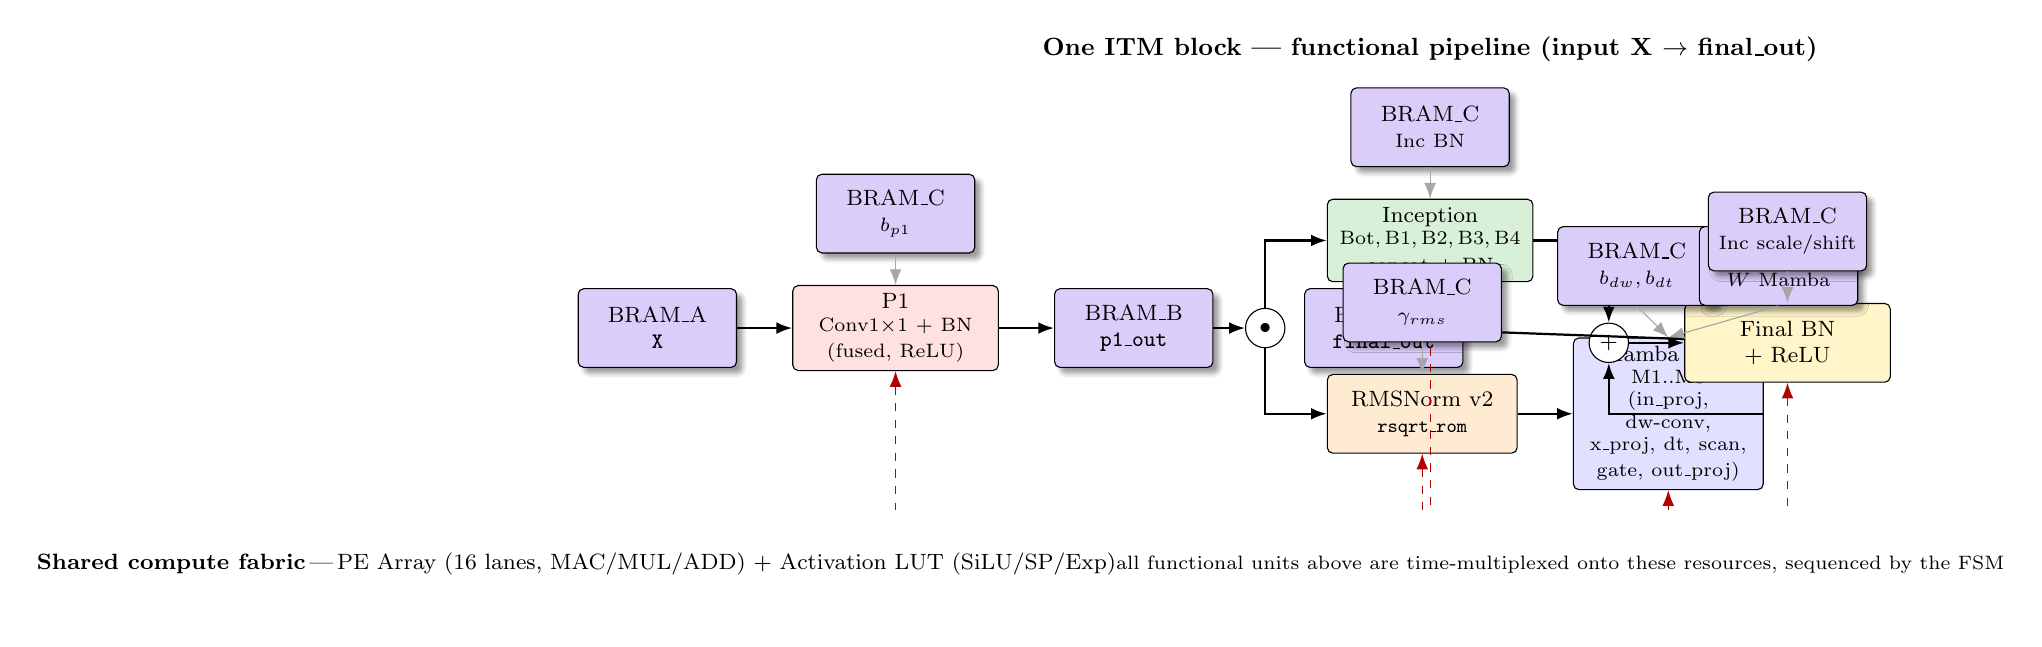
\begin{tikzpicture}[
    font=\footnotesize,
    >={Latex[length=2mm]},
    node distance=5mm and 7mm,
    blk/.style    ={draw, rounded corners=2pt, align=center,
                    text width=22mm, minimum height=10mm, inner sep=3pt},
    p1/.style     ={blk, fill=p1clr,  text width=24mm},
    incblk/.style ={blk, fill=incclr, text width=24mm},
    rms/.style    ={blk, fill=rmsclr, text width=22mm},
    mam/.style    ={blk, fill=mamclr, text width=22mm},
    fin/.style    ={blk, fill=finclr, text width=24mm},
    mem/.style    ={blk, fill=memclr, blur shadow={shadow blur steps=4},
                    text width=18mm},
    op/.style     ={draw, circle, fill=white, inner sep=1pt, minimum size=5mm,
                    font=\footnotesize},
    region/.style ={draw, rounded corners=4pt, dashed, line width=0.5pt,
                    inner sep=8pt},
    shared/.style ={draw, rounded corners=3pt, fill=shareclr,
                    align=center, inner sep=5pt},
    flow/.style   ={->, thick},
    busin/.style  ={<-, dashed, red!70!black},
]

% =============== Input / Output BRAM regions ===============
\node[mem]                (ramX)  {BRAM\_A\\ \texttt{X}};
\node[mem, right=72mm of ramX] (ramY) {BRAM\_A\\ \texttt{final\_out}};

% =============== P1 stage ===============
\node[p1, right=of ramX] (p1) {P1\\ \scriptsize Conv$1{\times}1$ + BN\\ \scriptsize (fused, ReLU)};

% =============== Intermediate p1_out in BRAM_B ===============
\node[mem, right=of p1] (ramP1) {BRAM\_B\\ \texttt{p1\_out}};

% =============== Split point ===============
\node[op, right=4mm of ramP1] (split) {$\bullet$};

% =============== Top branch — Inception (5 sub-branches collapsed) ===============
\node[incblk, above right=4mm and 6mm of split] (inc) {Inception\\ \scriptsize Bot,\,B1,\,B2,\,B3,\,B4\\ \scriptsize concat + BN};

% =============== Bottom branch — RMSNorm + Mamba ===============
\node[rms,  below right=4mm and 6mm of split] (rmsn) {RMSNorm v2\\ \scriptsize \texttt{rsqrt\_rom}};
\node[mam,  right=of rmsn] (mam) {Mamba SSM\\ \scriptsize M1..M8\\ \scriptsize (in\_proj, dw-conv,\\ \scriptsize x\_proj, dt, scan,\\ \scriptsize gate, out\_proj)};

% =============== Sum + Final BN ===============
\node[op, right=of inc, yshift=-13mm] (sum) {$+$};
\node[fin, right=of sum] (fin) {Final BN\\ + ReLU};

% =============== Wires ===============
\draw[flow] (ramX) -- (p1);
\draw[flow] (p1)   -- (ramP1);
\draw[flow] (ramP1) -- (split);
\draw[flow] (split.north) |- (inc.west);
\draw[flow] (split.south) |- (rmsn.west);
\draw[flow] (rmsn) -- (mam);
\draw[flow] (inc.east) -| (sum.north);
\draw[flow] (mam.east) -| (sum.south);
\draw[flow] (sum)  -- (fin);
\draw[flow] (fin)  -- (ramY);

% =============== Shared compute (bottom) ===============
\begin{scope}[on background layer]
  \node[shared, fit=(ramX)(ramY), yshift=-30mm,
        minimum width=140mm, minimum height=12mm] (shared) {};
\end{scope}
\node at (shared)
  {\textbf{Shared compute fabric}\,---\,PE Array (16 lanes, MAC/MUL/ADD) + Activation LUT (SiLU/SP/Exp)\\
   {\scriptsize all functional units above are time-multiplexed onto these resources, sequenced by the FSM}};

% Vertical dashed connector — each stage uses the shared fabric
\foreach \n in {p1, inc, rmsn, mam, fin}{%
  \draw[busin] (\n.south) -- (\n.south |- shared.north);
}

% =============== Const memory feeders (BRAM_C) ===============
\node[mem, above=4mm of p1] (cP1) {BRAM\_C\\ \scriptsize $b_{p1}$};
\node[mem, above=4mm of inc] (cInc) {BRAM\_C\\ \scriptsize Inc BN};
\node[mem, above=4mm of rmsn] (cR) {BRAM\_C\\ \scriptsize $\gamma_{rms}$};
\node[mem, above=4mm of mam, xshift=-4mm] (cM) {BRAM\_C\\ \scriptsize $b_{dw},b_{dt}$};
\node[mem, above=4mm of mam, xshift=14mm] (wM) {BRAM\_W\\ \scriptsize $W$ Mamba};
\node[mem, above=4mm of fin] (cF) {BRAM\_C\\ \scriptsize Inc scale/shift};

\foreach \src/\dst in {cP1/p1, cInc/inc, cR/rmsn, cM/mam, wM/mam, cF/fin}{%
  \draw[->, gray!70] (\src.south) -- (\dst.north);
}

% =============== Title bar ===============
\node[font=\bfseries\small, above=2mm of cInc] (ttl)
      {One ITM block --- functional pipeline (input X $\rightarrow$ final\_out)};

\end{tikzpicture}
\end{document}
